\section{Introduction}

In the early 1930s, experiments revealed contradictions in the resistance of certain metals in the low energy regime~\cite{Meissner_1930}. In particular, the expectation at the time was that the resistance should monotonically decrease, since it is directly related to electron-phonon interactions/scattering, which decrease with decreasing temperature. However, it was found that this is not the case; in fact, the resistance of these metals reached a minimum at some temperature and then started increasing again (see Fig.~\ref{fig:classickondo} for this behavior in gold). It eventually became clear that this was due to magnetic impurities in these particular metals.

\begin{figure}[ht]
  \centering
  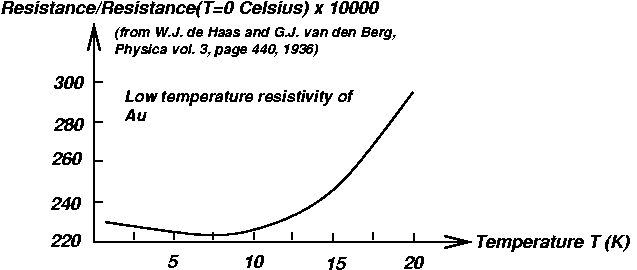
\includegraphics[width=0.6\linewidth]{../resources/gfx/classickondo.png}
  \caption{Figure created using the resistivity measurements found in Ref.~\cite{DeHaas_1936}.}
  \label{fig:classickondo}
\end{figure}

At this point, a number of models were introduced in an attempt to describe a system with metallic impurities, a couple of which being the Anderson model and the s-d exchange model. These were very simple models and only account for some of the behavior observed in experiment. In 1964, one major breakthrough occurred when Jun Kondo formulated the problem as a model in which the spin of the conduction electrons interacted with that of the magnetic impurity.\footnote{He didn't declare \textit{where} the spin moment came from, only that it was there; Anderson's model, as we will see, attempts to explain where it comes from.} The Hamiltonian he formulated for this system looks like:

\begin{equation}
  \hat{H} = \sum_{\vv{k},\sigma} \epsilon_{\vv{k}}c_{\vv{k},\sigma}^\dagger c_{\vv{k},\sigma} + J\sum_{\vv{k},\vv{k}',\alpha,\beta} c_{\vv{k},\alpha}^\dagger \vv{\sigma}_{\alpha,\beta} c_{\vv{k}',\beta} \cdot \vv{S},\label{eq:kondo-hamiltonian}
\end{equation}

where $c_{\vv{k},\sigma}^\dagger$ and $c_{\vv{k},\sigma}$ are the creation and annihilation operators for Bloch states representing the conduction electrons with a wavevector $\vv{k}$ and spin $\sigma$, $\epsilon_{\vv{k}}$ is the energy eigenvalue, $\vv{S}$ is the spin of the impurity, and $J$ is the coupling strength. Kondo then applied perturbation theory with this spin-spin interaction as the perturbation up to third order and retrieved results~\cite{Kondo_1964} which matched quite well with experiment; a functional form for the resistance goes like:

\begin{equation}
  R(T) = aT^5 + c_{\mathrm{imp}}R_0 - c_{\mathrm{imp}}R_1 \ln\left( \frac{k_B T}{D} \right),
\end{equation}

with the first term coming from the expected electron-phonon interactions and the second and third terms coming from perturbation theory related to the impurity. The logarithmic term did indeed successfully account for the resistance minimum and subsequent increasing as temperature decreased, but obviously, at a certain point it diverges. The point at which this singular behavior starts dominating is called the \textit{Kondo temperature} $T_K$, given roughly by

\begin{equation}
  k_BT_K \approx D\exp\left[ -\frac{1}{2J\rho} \right],\label{eq:kondo-temperature}
\end{equation}

with $D$ being the band width for the conduction electrons and $\rho$ being the density of states.

Evidently, despite accurately providing results in a particular low temperature regime, Kondo's solution wasn't perfect, and a better model was required in order to explain impurities in metals for temperatures at and below the Kondo temperature. This issue was henceforth dubbed ``The Kondo Problem''.


\subsection{Subsequent Notable Breakthroughs}

Soon afterwards, Philip Anderson introduced what was effectively a modifed renormalization scheme dubbed ``poor man's scaling''~\cite{Anderson_1970}. The essential recipe was a continuous scaling of the cutoff energy along with integrating out higher energy effects such that only the lower energy contributions remained, yielding an effective Hamiltonian valid at a lower energy. The effective Hamiltontian it yielded was of the same form as the previously unscaled one; the assumption that this same form would hold for the new system was an assumption, but turned out to work well. The reason for its name was that Anderson's scaling method wasn't quite how traditional renormalization schemes were typically conducted.

Unfortunately, so too did Anderson's scaling approach fail in the very low temperature regime. The reason for this was that upon successive scalings of the energy, the coupling strength between the impurity and the conduction electrons increased without bound -- it was \textit{renormalized}. This was an issue because the scaling method was in part possible due to a perturbative expansion about this coupling. Once this parameter was no longer small, the perturbative scheme no longer worked. This, again, yielded a non-zero temperature below which results were not accurate.

\begin{figure}[ht]
  \centering
  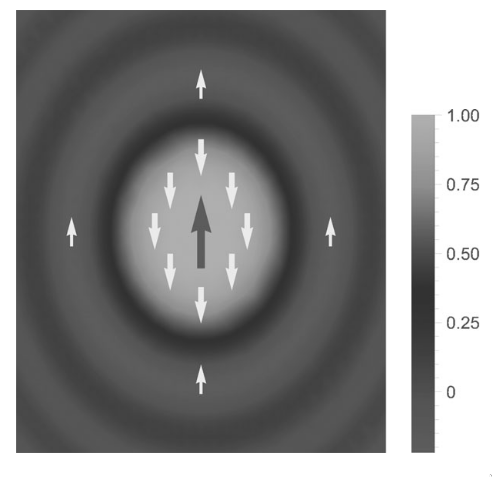
\includegraphics[width=0.35\linewidth]{../resources/gfx/kondo-cloud.png}
  \caption{The Kondo cloud, representing the induced spin density due to the bound state of the impurity and conduction electron bound state.}
  \label{fig:kondo-cloud}
\end{figure}

However, despite this method not yielding results all the way to $T=0$, its qualitative results were very significant. The fact that the coupling increased without bound indicated that the impurity and the conduction electrons formed a bound state. Other conduction electrons then screen this bound state, leading to an induced spin density that many like to call the Kondo cloud (see Fig.~\ref{fig:kondo-cloud}). Crudely summarizing, at higher energies the typical electron-phonon interactions dominate since they go like $T^5$. Then, they reach a minimum, after which the increasing coupling between the impurity and the conduction electrons form a singlet and induce a spin density that screens the singlet, which, roughly speaking, increases the resistance as the bound state forms a scattering center.

Kenneth Wilson eventually took inspriation from this approach and utilized a method derived from the numerical renormalization group (NRG)~\cite{Wilson_1975}, which did not involve perturbative expansion about a coupling that grew without bound, but rather about a generic small parameter $\Lambda$ related to the energy scaling factor, which remained small through the renormalization procedure. Because of this, Wilson's method was accurate at all energy scales, and finally produced coherent results for many properties at these energy scales, as well as confirming the qualitative result reached by Anderson and understanding how it is interpreted in NRG language.

As a connection to high-energy physics, this concept of a coupling increasing without bound is sort of a inverse \textit{asymptotic freedom} that we observe with quarks. In the latter case, the strong force (the coupling between the quarks) \textit{decreases} to zero at higher energies. At sufficient energies, our perturbative formalism becomes better and better. Consequently, this means the coupling \textit{increases} at \textit{lower} energies, meaning our perturbative formalism becomes inadequate. Methods like lattice QCD are being studied which have been effective so far at generating results at energies in which the coupling is too large to apply perturbation theory.


%%% Local Variables:
%%% mode: LaTeX
%%% TeX-master: "../project"
%%% End:
